\documentclass[letterpaper,12pt]{report}
\usepackage[top=1in,right=1in,bottom=1in,left=1.5in,nohead,nofoot]{geometry}

% PACKAGES
%**********
\usepackage{amsmath}		% AMS Math (http://www.ams.org/tex/amslatex.html)
\usepackage{amssymb}		% AMS Symbols
\usepackage{amsthm}			% AMS Theorems
\usepackage{tocloft}		% Format the Table of Contents
\usepackage{float}			% More float commands
\usepackage{sectsty}		% Format section and chapter headings
\usepackage{graphicx}		% Insert images in eps or pdf format
\usepackage{setspace}		% Line-spacing

% Potentially useful packages:
% \usepackage{epsfig}			% For EPS figures
% \usepackage{subfigure}		% For side-by-side figures
% \usepackage{sidecap}		% Put captions on the side of figures
% \usepackage{rotating}		% Rotatiion of figures and tables
% \usepackage{multirow}		% Column and row spanning in tables
% \usepackage{chapterbib}		% Insert bibliograhpy with a simple include command

% Generally, you will not want to edit this file, unless adding a LIST OF ILLUSTRATIONS (or similar)

\renewcommand\contentsname{TABLE OF CONTENTS}
\setlength{\cftbeforetoctitleskip}{0in}
\renewcommand{\cfttoctitlefont}{\hspace{\fill}\large\bfseries}
\renewcommand{\cftaftertoctitle}{\hspace{\fill}}

\renewcommand\listtablename{LIST OF TABLES} % Defines exact text of Title
\setlength{\cftbeforelottitleskip}{1in} % Defines how far down from the margin the title should be placed
\setlength{\cftafterlottitleskip}{0.25in} % Defines how far below the title the first entry will be
\renewcommand{\cftlottitlefont}{\hspace{\fill}\large\bfseries} % This line and the next define that the title should be centered and followed by a line with 'Table' on the left and 'Page' on the right.
\renewcommand{\cftafterlottitle}{\hspace{\fill} \vskip 10mm {\large Table \hspace{\fill} Page}}

\renewcommand\listfigurename{LIST OF FIGURES}
\setlength{\cftbeforeloftitleskip}{1in}
\setlength{\cftafterloftitleskip}{0.25in}
\renewcommand{\cftloftitlefont}{\hspace{\fill}\large\bfseries}
\renewcommand{\cftafterloftitle}{\hspace{\fill} \vskip 10mm {\large Figure \hspace{\fill} Page}}

\renewcommand\cftpartdotsep{\cftdotsep}
\renewcommand\cftchapdotsep{\cftdotsep}
\renewcommand\cftsecdotsep{\cftdotsep}
\renewcommand\cftsubsecdotsep{\cftdotsep}
\renewcommand\cftsubsubsecdotsep{\cftdotsep}
\renewcommand\cftparadotsep{\cftdotsep}
\renewcommand\cftsubparadotsep{\cftdotsep}
\renewcommand\cftfigdotsep{\cftdotsep}
\renewcommand\cfttabdotsep{\cftdotsep}

\setlength{\cftbeforepartskip}{12pt}
\setlength{\cftbeforechapskip}{12pt}
\setlength{\cftbeforesecskip}{12pt}
\setlength{\cftbeforesubsecskip}{12pt}
\setlength{\cftbeforesubsubsecskip}{12pt}
\setlength{\cftbeforeparaskip}{12pt}
\setlength{\cftbeforesubparaskip}{12pt}
	% Lots of special formatting to make the ToC adhere to MU requirements

\begin{document}

\doublespacing % Double line-spacing ( or specify something like \setspacing{1.8} )
\allsectionsfont{\singlespacing} % Only body text needs double spacing, titles can be single spaced

\setcounter{page}{1}    
\pagenumbering{roman}

\thispagestyle{empty}

\vspace*{\fill}
\centerline{\large{\bf THE TITLE OF YOUR}} % The title on the Title Page must be in all caps.
\centerline{\large{\bf PROJECT GOES HERE}}
\vskip 10mm
\centerline{\rule{150mm}{0.2mm}} % You can adjust the length of the horizontal line here.
\vskip 10mm
\centerline{A Thesis presented to} % Choose Thesis or Dissertation
\centerline{the Faculty of the Graduate School}
\centerline{at the University of Missouri}
\vskip 10mm
\centerline{\rule{150mm}{0.2mm}}
\vskip 10mm
\centerline{In Partial Fulfillment}
\centerline{of the Requirements for the Degree}
\centerline{Doctor of Philosophy} % Change to your degree
\vskip 10mm
\centerline{\rule{150mm}{0.2mm}}
\vskip 10mm
\centerline{by}
\centerline{YOUR NAME} % Your name on the Title Page must be in all caps.
\centerline{Dr. Advisor Name, Thesis Supervisor} % Edit advisor and choose Thesis or Dissertation
\centerline{MAY 2005} % The month is required to be capitalized.  Use the month and year of your graduation, not the month and year you defend.
\vspace*{\fill}
	% Input the Title Page (no page number, but counts as roman numeral 'i')
\newpage
\thispagestyle{empty}

The undersigned, appointed by the Dean of the Graduate School, have 
examined the dissertation entitled: % Choose thesis or dissertation

\vspace{8mm}
\centerline{THE TITLE OF YOUR} % The title on the Title Page must be in all caps.
\centerline{PROJECT GOES HERE}
\vspace{8mm}
\noindent presented by Your Name, % Edit with your name (does not need to be in all caps.)

\noindent a candidate for the degree of Doctor of Philosophy % Change to your degree
and hereby certify that, in their opinion, it is worthy of acceptance.
\vskip 15mm
\centerline{\rule{100mm}{0.2mm}}
\centerline{Dr. Advisor Name} % Edit advisor
\vskip 10mm
\centerline{\rule{100mm}{0.2mm}}
\centerline{Dr. Committee Member} % Edit committee member 1
\vskip 10mm
\centerline{\rule{100mm}{0.2mm}}
\centerline{Dr. Committee Member} % Edit committee member 1
\vskip 10mm
\centerline{\rule{100mm}{0.2mm}}
\centerline{Dr. Committee Member} % Edit committee member 1
\vskip 10mm
\centerline{\rule{100mm}{0.2mm}}
\centerline{Dr. Committee Member} % Edit committee member 1
	% Input the Approval Page (no page number)
\newpage
\pagenumbering{roman}
\setcounter{page}{2}
\addcontentsline{toc}{chapter}{ACKNOWLEDGMENTS} % This is the American english spelling (no E between G and M)

\centerline{\bf \large ACKNOWLEDGMENTS}
\vskip 10mm % Edit everything below with your acknowledging text.
This page is where you would acknowledge all those who helped you with your academic research. This is not necessarily where you would recognize loved ones who supported you during your studies. That would be more appropriately done in an optional Dedication page. I would like to thank Professor Smith � Lorem ipsum dolor sit amet, consectetuer adipiscing elit. Vestibulum eu tellus. Nullam et odio eget sapien porttitor interdum. Donec vel ante. Maecenas in sem a nunc viverra hendrerit. Quisque ut massa quis pede blandit pharetra. \par
Pellentesque sed ligula sit amet ligula scelerisque sagittis. Nulla adipiscing tellus at pede. Cras id nunc vel diam congue dictum. Donec a nulla nec eros ornare consequat. Nullam quis orci. Nam adipiscing, erat in congue pellentesque, dolor eros euismod quam, a egestas mauris magna varius justo. \par
Sed eu sem et lorem blandit volutpat. Duis pulvinar, arcu quis suscipit convallis, ante elit auctor dui, in fermentum diam velit a mauris. In risus odio, consectetuer quis, ullamcorper in, rutrum ut, metus.
	% Input the Acknowledgement Page (roman numeral page number 'ii')
% Only edit this file if you want to include a new list of illustrations, theorems, or other (in which case you will need to add a block to Command_Mods.tex

% Generate a table of contents
\newpage
\singlespacing
\tableofcontents
\doublespacing

% Generate a list of Tables and a list of Figures:
\newpage
\addcontentsline{toc}{chapter}{LIST OF TABLES}
\listoftables

\newpage
\addcontentsline{toc}{chapter}{LIST OF FIGURES}
\listoffigures
	% Generate and input a Table of Contents and List of Figures/Tables/etc.(roman numeral page number 'iii')

\newpage
\addcontentsline{toc}{chapter}{ABSTRACT}

\centerline{\bf \large ABSTRACT}
\vskip 10mm % Edit everything below with your acknowledging text.
This is the abstract of your dissertation project.  It should not exceed one page.

\newpage
\setcounter{page}{1}
\pagenumbering{arabic}
\addtocontents{toc}{\protect \contentsline {chapter}{CHAPTER}{}}

\chapter{Introduction}
	\label{CH_Intro}

Introduce the reader to the current problem that you wish to solve, and why anyone should care about it.
\chapter{Title of second chapter}
	\label{CH_02}

\section{Title of section}
The introduction counts as chapter 1.  This page shows how the bulk of your thesis will be organized: through chapters and sections. Here is a citation.\cite{OBTMBD01}

\subsection{Title of subsection}
Here is a subsection.  The guidelines say that quotations of four lines or longer should be single spaced with the left and right margins indented, here's how this looks:\par

\singlespacing
\begin{quotation}
``Lorem ipsum dolor sit amet, consectetuer adipiscing elit. Vestibulum eu tellus. Nullam et odio eget sapien porttitor interdum. Donec vel ante. Maecenas in sem a nunc viverra hendrerit. Quisque ut massa quis pede blandit pharetra." \par
``Pellentesque sed ligula sit amet ligula scelerisque sagittis. Nulla adipiscing tellus at pede. Cras id nunc vel diam congue dictum. Donec a nulla nec eros ornare consequat. Nullam quis orci. Nam adipiscing, erat in congue pellentesque, dolor eros euismod quam, a egestas mauris magna varius justo."
\end{quotation}
\doublespacing

\section{Mathematics}
Here is how to display some in-line math, $x=\cos\theta$. Here is a numbered equation:
\begin{equation} \label{eq:01}
	\sum\limits_{k=0}^{\infty}{\frac{1}{k}}.
\end{equation}
\chapter{Title of third chapter}
	\label{CH_03}


\section{This is an example section title which will span two lines both here and in the table of contents}
Further illustration of how chapters are presented.


\subsection{Title of subsection}
Here is a subsection.  The following figure will show up in the `List of Figures'.

\begin{figure}[h] % h places the image 'here' (as long as LaTeX thinks it will fit here well), 't' for top of page, 'b' for bottom of page, 'H' for I WANT IT HERE!!! (regardless of whether the latex compiler thinks it will fit.)
	\centering
	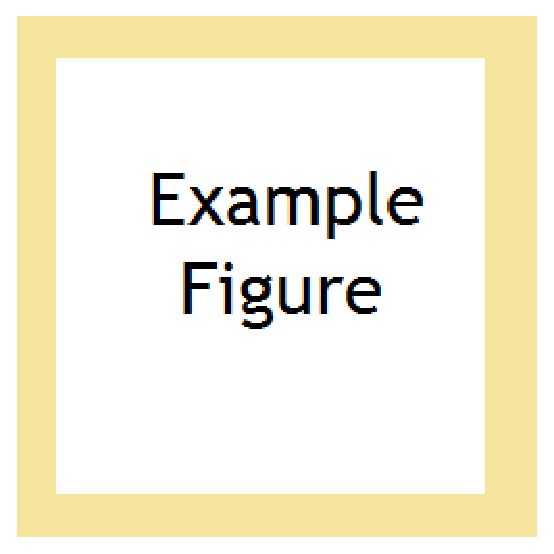
\includegraphics[width=2.0in]{Figures/figure1}
	\caption[Box figure]{A sample image which will show up in the the List of Figures as `Box figure'}
\end{figure}
\begin{table}[t]
	\centering
	\begin{tabular}{|r|l|}
	\hline
	7C0 & hexadecimal \\
	3700 & octal \\ \cline{2-2}
	11111000000 & binary \\
	\hline \hline
	1984 & decimal \\
	\hline
	\end{tabular}
	\caption[Digit representation]{A sample table which will show up in the the List of Tables as `Digit representation table'; it is set to align at the top of a page}
\end{table}

Some paragraph text follows. Some paragraph text follows. Some paragraph text follows. Some paragraph text follows. Some paragraph text follows. Some paragraph text follows. Some paragraph text follows. Some paragraph text follows. Some paragraph text follows. Some paragraph text follows. Some paragraph text follows. Some paragraph text follows. Some paragraph text follows. Some paragraph text follows. Some paragraph text follows. Some paragraph text follows. Some paragraph text follows. Some paragraph text follows. 

\begin{table}[h]
	\centering
	\begin{tabular}{llr}
	\hline
	\multicolumn{2}{c}{Item} \\
	\cline{1-2}
	Animal & Description & Price (\$) \\
	\hline
	Gnat  & per gram & 13.65 \\
	 & each     &  0.01 \\
	Gnu   & stuffed  & 92.50 \\
	Emu   & stuffed  & 33.33 \\
	Armadillo & frozen & 8.99 \\
	\hline
	\end{tabular}
	\caption[Odd foods]{Another table which will show up in the the List of Tables as `Odd foods'; it is set to align ``here" in the text.}
\end{table}




\chapter{Summary and concluding remarks}
	\label{CH_summary}

Congratulations on completing your dissertation.

\newpage
\addcontentsline{toc}{chapter}{APPENDIX}
\appendix

\chapter{Title of first appendix}
	\label{AP_01}

\section{Section title}
Here is some additional information which would have detracted from the point being made in the main article.
\subsection{Subsection title}
This section even has subtitles
\newpage
\addcontentsline{toc}{chapter}{BIBLIOGRAPHY}
\printbibliography

\newpage
\addcontentsline{toc}{chapter}{VITA}

\centerline{\bf \large VITA}
\vskip 10mm % Edit everything below with your acknowledging text.
This is a summary of your {\it professional} life, and should be written appropriately.  This can be written in the following order:  where your where born, what undergraduate university you graduated from, if you received a masters, and which institution you graduated from with your PhD (University of Missouri).  You can describe when you began research with your current advisor. \par
In another paragraph, you could say if/when you were married, what the name of your kids are, and what your plans are for after graduation if you choose.  Take a look at other vita's from other dissertations for examples.


\end{document}